% User guide for the AMC web portal (amc.rjana.in), for teachers who have
% never used AMC. Build with `make` (latexmk, pdflatex). The screenshots
% come from capture/capture.mjs (see capture/README.md).
\documentclass[11pt]{article}
\usepackage{amcguide}

% The amc-webapp version this edition's screenshots show (amc-webapp.version).
\usepackage{catchfile,xstring}
\CatchFileDef{\appversionfull}{amc-webapp.version}{\endlinechar=-1}
\StrLeft{\appversionfull}{7}[\appversion]
\newcommand\edition{November 2026}

\newcommand\portal{\href{https://amc.rjana.in}{\texttt{amc.rjana.in}}}
\newcommand\demouser{\texttt{demo\_instructor}}
\newcommand\demopass{\texttt{Demo@1234!4567}}

\hypersetup{pdftitle={AMC web portal: user guide},pdfauthor={Rakesh Jana},
  pdfsubject={Multiple-choice exams from the questions to the marked sheets}}

\begin{document}

% ====================================================================== cover
\begin{titlepage}
\thispagestyle{empty}
\begin{tikzpicture}[remember picture,overlay]
  \fill[brand] (current page.north west) rectangle ([yshift=-118mm]current page.north east);
  \fill[brandink] ([yshift=-118mm]current page.north west) rectangle ([yshift=-121mm]current page.north east);
  \node[anchor=north west,text=white,font=\small\bfseries,inner sep=0pt] at ([xshift=20mm,yshift=-22mm]current page.north west)
    {AMC WEB PORTAL \quad\textbullet\quad \texttt{amc.rjana.in}};
  \node[anchor=north west,text=white,font=\fontsize{46}{50}\selectfont\bfseries,inner sep=0pt] at ([xshift=20mm,yshift=-36mm]current page.north west)
    {User guide};
  \node[anchor=north west,text=white,font=\Large,text width=150mm,inner sep=0pt,align=left] at ([xshift=20mm,yshift=-60mm]current page.north west)
    {Multiple-choice exams from the first question to the marked answer sheets, step by step.};
  \node[anchor=north west,text=white!85!brand,font=\normalsize,text width=150mm,inner sep=0pt,align=left,execute at begin node={\hyphenpenalty=10000\relax}] at ([xshift=20mm,yshift=-84mm]current page.north west)
    {For teachers using the portal for the first time. No knowledge of AMC, LaTeX or programming needed.};
  \node[anchor=north,inner sep=0pt,drop shadow={opacity=0.35,shadow xshift=1.2mm,shadow yshift=-1.2mm}] at ([yshift=-134mm]current page.north)
    {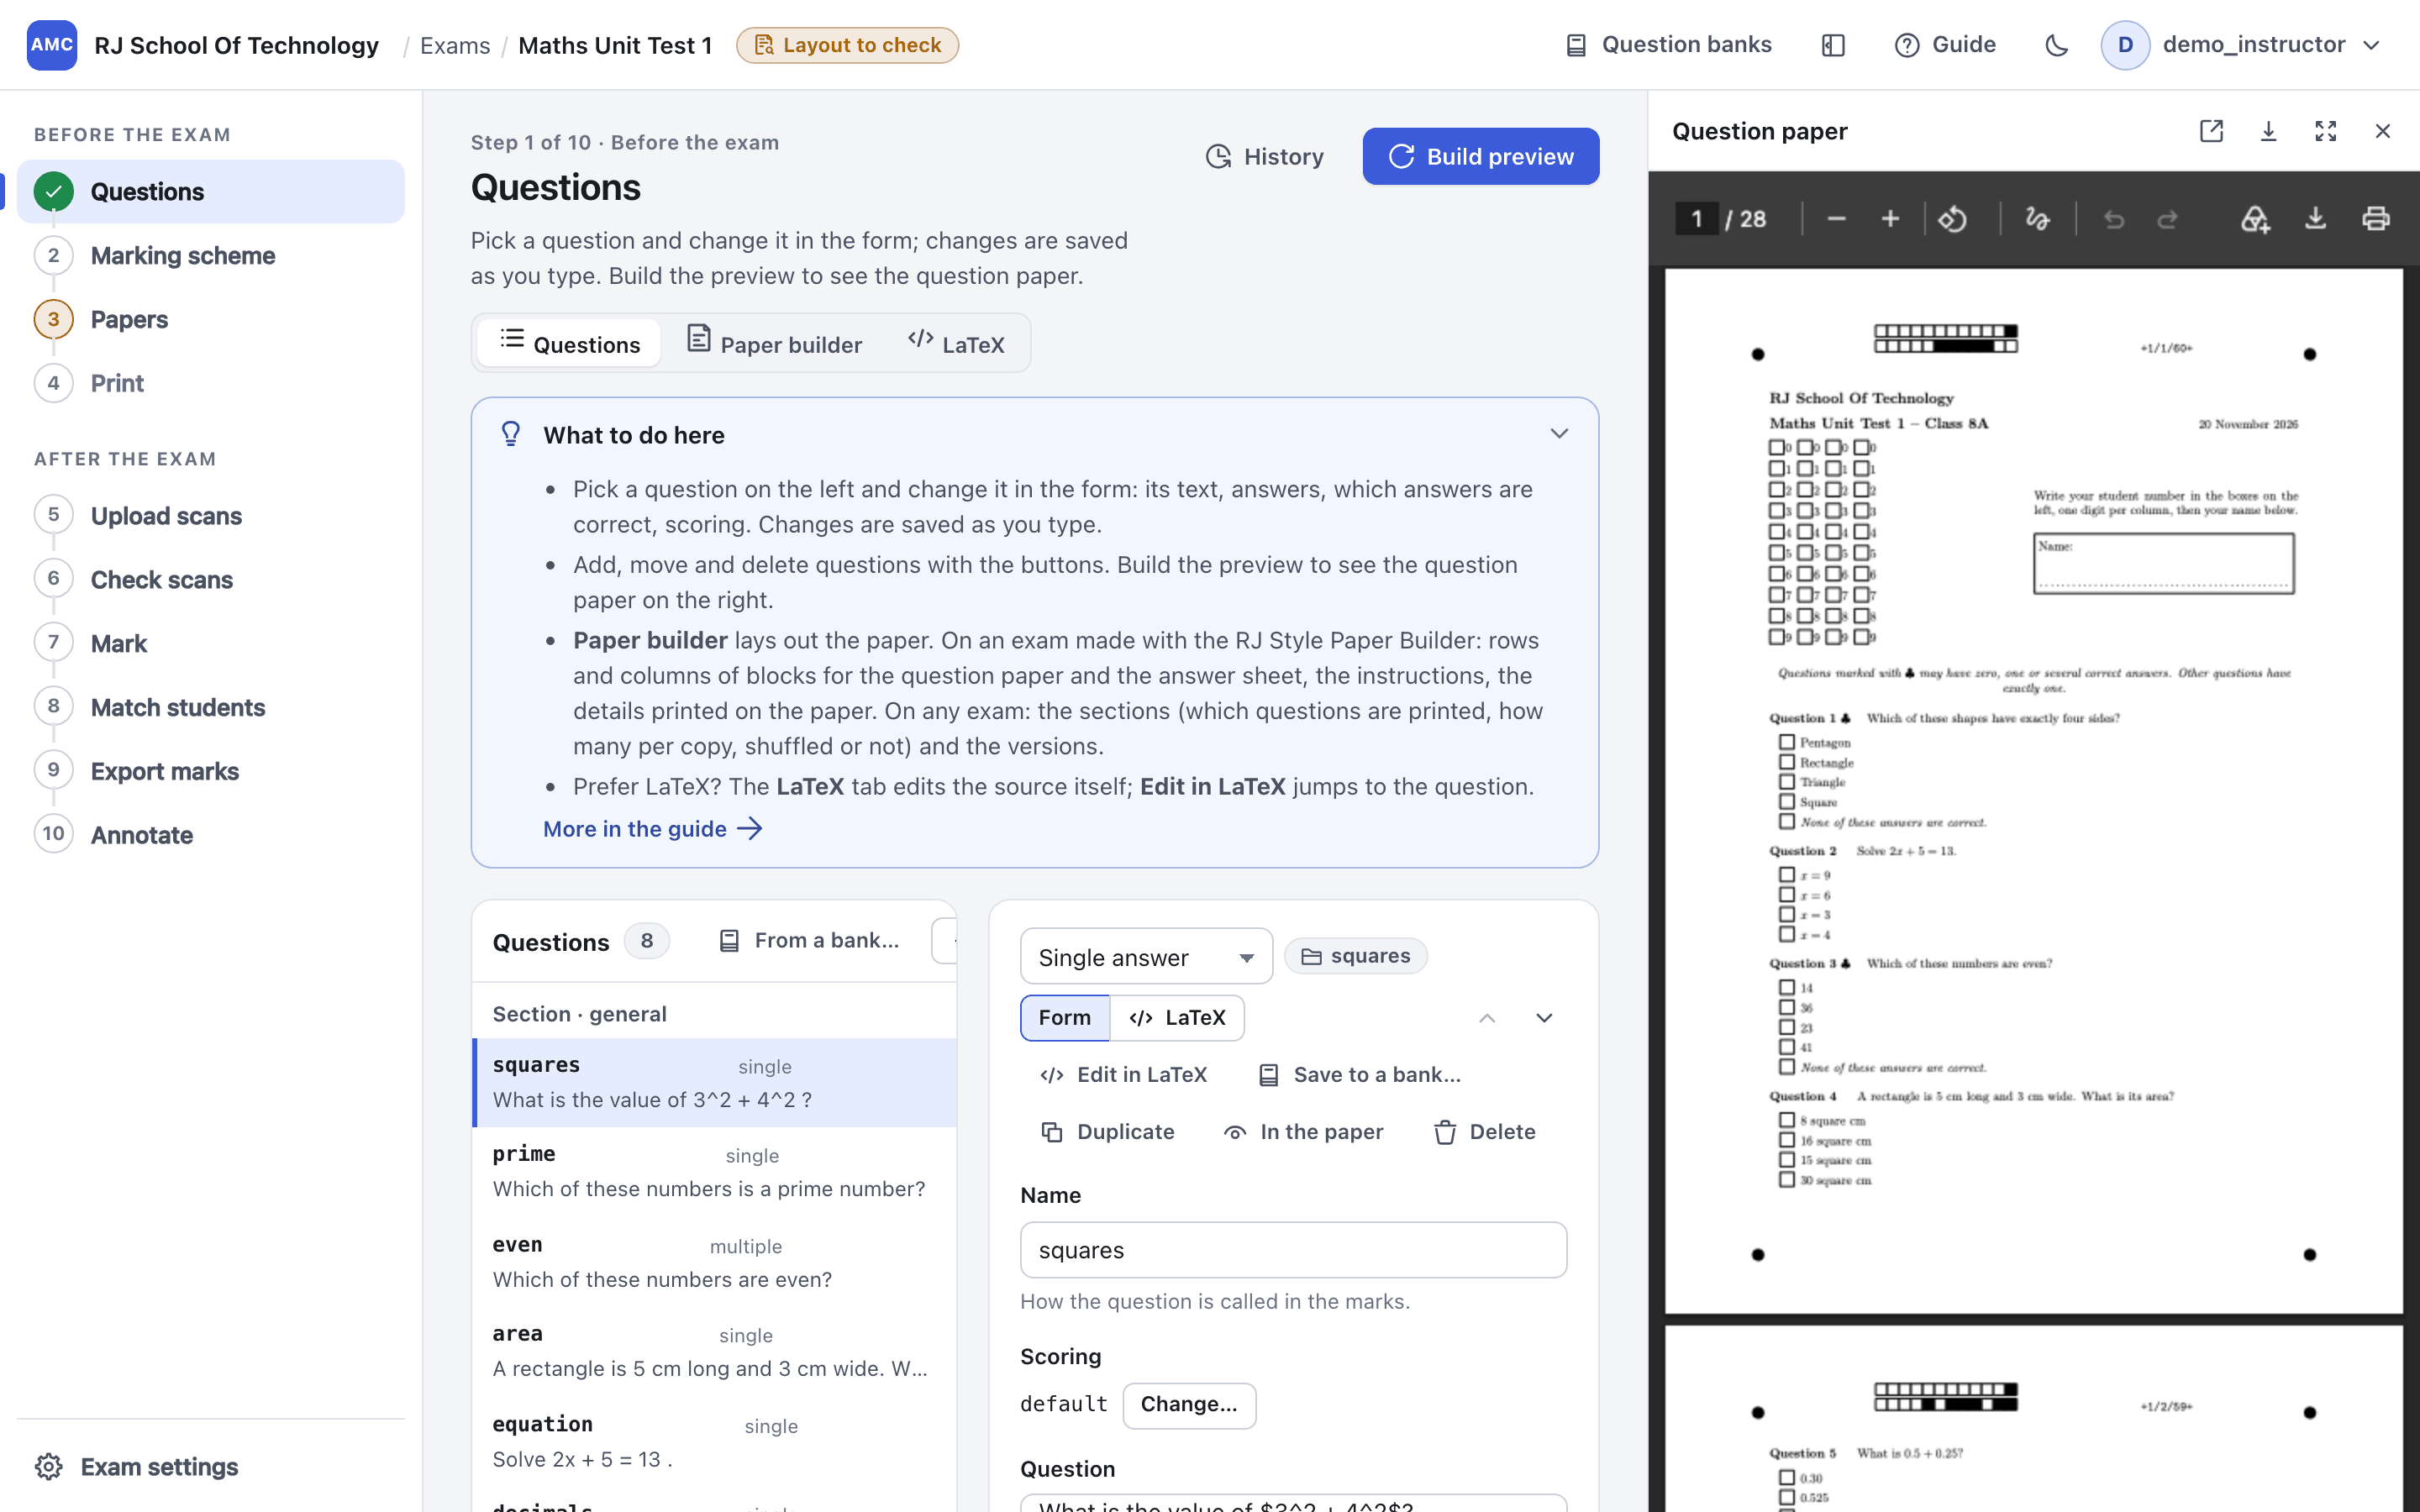
\includegraphics[width=150mm]{screenshots/workspace}};
  \node[anchor=south,fill=white,draw=brand,line width=1pt,rounded corners=4pt,text width=146mm,inner sep=7pt,align=left,font=\small]
    at ([yshift=24mm]current page.south) {%
    \textbf{\color{brand}Try it now.}\quad Open \textbf{\portal} and sign in with the demo account:\\[3pt]
    \begin{tabular}{@{}ll@{}}Username & \demouser\\ Password & \demopass\end{tabular}};
  \node[anchor=south,text=muted,font=\footnotesize] at ([yshift=12mm]current page.south) {\edition{} edition \textbullet{} portal version \texttt{\appversion}};
\end{tikzpicture}
\end{titlepage}

% ====================================================================== contents
\pagestyle{plain}
{\hypersetup{linkcolor=ink}\setcounter{page}{2}
\noindent{\fontsize{20}{24}\selectfont\bfseries\color{brandink}Contents}\par\vspace{2pt}{\color{line}\rule{\linewidth}{0.8pt}}\par\medskip
\makeatletter\@starttoc{toc}\makeatother}
\clearpage
\pagestyle{fancy}

% ====================================================================== 1
\section{Welcome}\label{sec:welcome}

\subsection{What the portal does}

The portal makes \textbf{multiple-choice exams that mark themselves}. It runs \textbf{AMC} (\emph{Auto Multiple Choice}), free software used by schools and universities for years, through simple pages in your web browser.

The idea fits in one picture:

\begin{center}
\begin{tikzpicture}[
  stage/.style={rounded corners=5pt,fill=#1!10,draw=#1,line width=0.8pt,minimum width=27mm,minimum height=24mm,align=center,font=\footnotesize,text width=25mm,execute at begin node={\hyphenpenalty=10000\relax}},
  num/.style={circle,fill=#1,text=white,font=\footnotesize\bfseries,minimum size=5.5mm,inner sep=0pt},
  arr/.style={-{Stealth[length=3mm]},line width=1.2pt,draw=muted}]
  \node[stage=before] (a) at (0,0) {\textbf{You write}\\the questions\\and answers};
  \node[stage=before] (b) at (3.35,0) {\textbf{The portal prints}\\one paper per student, with boxes};
  \node[stage=warn] (c) at (6.7,0) {\textbf{Students tick}\\the boxes with a dark pen};
  \node[stage=after] (d) at (10.05,0) {\textbf{You scan}\\the answer sheets and upload them};
  \node[stage=after] (e) at (13.4,0) {\textbf{The portal marks}\\every sheet and makes the results};
  \foreach \x/\y in {a/b,b/c,c/d,d/e} \draw[arr] (\x) -- (\y);
  \foreach \n/\c/\t in {a/before/1,b/before/2,c/warn/3,d/after/4,e/after/5} \node[num=\c] at (\n.north west) {\t};
\end{tikzpicture}
\end{center}

You get a \textbf{spreadsheet of marks}, and for each student a \textbf{marked copy of their answer sheet}, showing which answers were right or wrong and the points for each question, ready to hand back. Nobody has to mark a single paper by hand.

\begin{why}[Why it works]
Each printed page carries small black dots in its corners and a code at the top. When a scanned page comes back, the portal uses them to recognise the page, straighten it, and find every box. A box is \emph{ticked} when it is dark enough. That is also why the papers must be printed exactly as the portal made them (at 100\,\%), and why the questions can't change once they are printed.
\end{why}

\needspace{0.72\textheight}
\subsection{Words you will meet}\label{sec:words}

\begin{panel}
\renewcommand{\arraystretch}{1.25}
\begin{tabularx}{\linewidth}{@{}>{\bfseries}p{33mm}X@{}}
Exam & Everything for one test: its questions, its papers, the scans and the marks. You can have as many as you like.\\
Copy & One student's paper. Each copy has its own number, and the questions and answers can be in a different order on each, so neighbours can't copy.\\
Question paper & What students read. The boxes to tick are next to the answers, or on a separate answer sheet.\\
Answer sheet & The page(s) with the boxes students tick. With a \emph{separate} answer sheet, all boxes are on one page at the end of each copy.\\
Answer key & Which answers are correct. You tick them while writing the questions.\\
Marking scheme & How ticks become points (and a final mark): for example 1 point for a right answer, minus 0.25 for a wrong one.\\
Layout & Where every box is on every page. The portal records it when it builds the papers and needs it to read the scans.\\
Scan & A picture (PDF, JPEG\ldots) of a page students wrote on, made with a scanner or a photocopier that scans.\\
Class list & A spreadsheet of your students, saved as a CSV file: one line per student, with a student number and a name.\\
Student number & The number a student writes on the paper by ticking digits in a grid. The portal reads it and finds the student in the class list.\\
Annotated sheet & A student's answer sheet with their ticks marked right or wrong and their mark written on it.\\
\end{tabularx}
\end{panel}

\subsection{What you need}

\begin{itemize}
  \item A \textbf{laptop or desktop computer} with a recent web browser (Chrome, Edge, Firefox or Safari). Tablets and phones aren't supported yet.
  \item An \textbf{A4 printer}, or a shop that prints PDF files.
  \item A \textbf{scanner}, or a photocopier that scans to PDF. Most office photocopiers can, through their document feeder.
  \item Your \textbf{class list} as a spreadsheet (optional, but it puts names next to the marks).
  \item An \textbf{account} on the portal, made by its administrator. To try things out, use the demo account below.
\end{itemize}

\subsection{Try it on the demo account}\label{sec:demo}

\begin{panel}[colframe=brand,boxrule=1pt]
\begin{tabular}{@{}l@{\hspace{6mm}}l@{}}
\textbf{Address} & \portal\\[2pt]
\textbf{Username} & \demouser\\[2pt]
\textbf{Password} & \demopass\\
\end{tabular}

\smallskip
The demo account is open to everyone who has this guide. Use it to follow the chapters below with your own clicks: create an exam, write a few questions, build the papers, and so on.
\end{panel}

\begin{careful}[Please]
The demo account is \textbf{shared}: other people see what you put in it, and it may be emptied from time to time. \textbf{Don't put real students' names or marks in it}, and \textbf{don't change its password}, or the next person can't sign in. For real exams, ask the administrator for your own account.
\end{careful}

\subsection{How to read this guide}

\begin{itemize}
  \item Words in \ui{dark blue bold} are written exactly as on the screen: buttons, tabs, fields.
  \item Red frames and numbered badges such as \badge{1} on a screenshot match the numbered list under it.
  \item \textcolor{brand}{$\rightarrow$}~links take you to another part of the guide with more detail. In the PDF, click them.
  \item Green boxes are tips; orange boxes are things to watch out for.
\end{itemize}

The screenshots show a demo exam, \emph{Maths Unit Test 1} for class 8A, taken from its first question to the marked sheets. Your screens will look the same, with your own exams in them.

% ====================================================================== 2
\section{Getting started}\label{sec:start}

\subsection{Sign in}

Open \portal{} in your browser. The sign-in page asks for your username and password.

\begin{keep}
\begin{guidefig}{The sign-in page.}
\begin{shot}[0.5\linewidth]{signin}
  \mk[w]{user}{1}\mk[w]{pass}{2}\mk[e]{go}{3}
\end{shot}
\end{guidefig}
\begin{callouts}
  \item Your \ui{Username}, for example \demouser.
  \item Your \ui{Password}. Capital and small letters count.
  \item \ui{Sign in}.
\end{callouts}
\end{keep}

\begin{tip}
After several wrong passwords the portal makes you wait a few minutes before trying again. If you have forgotten your password, ask the administrator: accounts are made and reset by them.
\end{tip}

\subsection{The Exams page}\label{sec:exams-page}

After signing in you land on \ui{Exams}, the list of your exams. The first time, it is empty.

\begin{keep}
\begin{guidefig}{The Exams page of a new account.}
\begin{shot}{dash-empty}
  \mk[s]{newexam}{1}\mk[n]{banks}{2}\mk[n]{guide}{3}\mk[n]{theme}{4}\mk[n]{account}{5}\mk[s]{trash}{6}\mk[s]{import}{7}
\end{shot}
\end{guidefig}
\begin{callouts}
  \item \ui{New exam} starts a new exam (\seesec{sec:create}).
  \item \ui{Question banks}: your own collections of questions to use again (\seesec{sec:banks}).
  \item \ui{Guide}: the portal's built-in help, one page per step.
  \item Light or dark colours.
  \item Your account: change your password, or sign out.
  \item \ui{Trash}: exams you deleted, kept for 30 days.
  \item \ui{Import an exam\ldots}: bring in an exam saved from this or another AMC installation.
\end{callouts}
\end{keep}

Clicking the school name at the top left always brings you back to this page.

\subsection{Your password, and signing out}

Open the menu with your name at the top right, then \ui{Account, password and sign out}. That page lets you set a new password and sign out. On a shared computer, always sign out when you leave.

\begin{guidefig}{The account menu.}
\begin{shot}[0.42\linewidth]{account-menu}
  \hl{item}
\end{shot}
\end{guidefig}

% ====================================================================== 3
\section{How an exam works: the ten steps}\label{sec:steps}

Every exam goes through the same ten steps: four before the exam, six after it. The portal lists them on the left of the screen and shows where each one stands. You can open any step at any time.

\begin{center}
\begin{tikzpicture}[
  st/.style={rounded corners=4pt,fill=#1!10,draw=#1,line width=0.7pt,minimum width=30mm,minimum height=13mm,align=center,font=\small\bfseries,text width=28mm},
  nb/.style={circle,fill=#1,text=white,font=\scriptsize\bfseries,minimum size=5mm,inner sep=0pt},
  ar/.style={-{Stealth[length=2.4mm]},line width=1pt,draw=muted}]
  \node[font=\footnotesize\bfseries,text=before,anchor=west] at (-1.6,1.15) {BEFORE THE EXAM};
  \foreach \i/\t [count=\k] in {1/Questions,2/Marking scheme,3/Papers,4/Print} {
    \node[st=before] (s\i) at ({(\k-1)*3.55},0) {\t};
    \node[nb=before] at (s\i.north west) {\i};
  }
  \foreach \a/\b in {1/2,2/3,3/4} \draw[ar] (s\a) -- (s\b);
  \node[rounded corners=4pt,fill=warn!12,draw=warn,line width=0.7pt,minimum width=30mm,minimum height=13mm,align=center,font=\small\bfseries,text width=28mm] (day) at (13.0,-1.75) {Exam day\\[-1pt]{\scriptsize\normalfont students tick boxes}};
  \draw[ar] (s4.east) -| (day.north);
  \node[font=\footnotesize\bfseries,text=after,anchor=west] at (-1.6,-2.45) {AFTER THE EXAM};
  \foreach \i/\t [count=\k] in {5/Upload scans,6/Check scans,7/Mark} {
    \node[st=after] (s\i) at ({9.0-(\k-1)*3.55},-3.5) {\t};
    \node[nb=after] at (s\i.north west) {\i};
  }
  \draw[ar] (day.south) |- (s5.east);
  \draw[ar] (s5) -- (s6); \draw[ar] (s6) -- (s7);
  \foreach \i/\t [count=\k] in {8/Match students,9/Export marks,10/Annotate} {
    \node[st=after] (s\i) at ({(\k-1)*3.55+1.9},-5.6) {\t};
    \node[nb=after] at (s\i.north west) {\i};
  }
  \draw[ar] (s7.south) -- (s8.north);
  \draw[ar] (s8) -- (s9); \draw[ar] (s9) -- (s10);
\end{tikzpicture}
\end{center}

\begin{panel}
\renewcommand{\arraystretch}{1.3}\small
\begin{tabularx}{\linewidth}{@{}>{\bfseries}l X >{\raggedleft\arraybackslash}p{17mm}@{}}
\toprule
Step & What you do & Details\\
\midrule
\textcolor{before}{1 Questions} & Write the questions and their answers, and tick the correct ones. & p.~\pageref{step:questions}\\
\textcolor{before}{2 Marking scheme} & Choose how many points a right or wrong answer gives, and the final mark. & p.~\pageref{step:marking}\\
\textcolor{before}{3 Papers} & Build the papers for every student and check that the boxes were found. & p.~\pageref{step:papers}\\
\textcolor{before}{4 Print} & Download the PDFs and print them. This locks the questions. & p.~\pageref{step:print}\\
\midrule
\textcolor{after}{5 Upload scans} & Upload the scanned answer sheets. & p.~\pageref{step:upload}\\
\textcolor{after}{6 Check scans} & Settle the few pages or boxes the portal wasn't sure about. & p.~\pageref{step:check}\\
\textcolor{after}{7 Mark} & Compute every student's mark with one click. & p.~\pageref{step:mark}\\
\textcolor{after}{8 Match students} & Put a name on each answer sheet, mostly automatically. & p.~\pageref{step:match}\\
\textcolor{after}{9 Export marks} & Download the marks as a spreadsheet. & p.~\pageref{step:export}\\
\textcolor{after}{10 Annotate} & Make each student's marked answer sheet to give back. & p.~\pageref{step:annotate}\\
\bottomrule
\end{tabularx}
\end{panel}

\subsection{The exam's workspace}\label{sec:workspace}

When you open an exam, the screen has the same parts in every step.

\begin{keep}
\begin{guidefig}{An exam open on its first step, Questions.}
\begin{shot}{workspace}
  \mk[ne]{before}{1}\mk[ne]{after}{2}\mk[se]{settings}{3}\mk[e]{top}{4}\mk[nw]{guide}{5}\mk[n]{tabs}{6}\mk[sw]{build}{7}\mk[nw]{preview}{8}
\end{shot}
\end{guidefig}
\begin{callouts}
  \item The four steps \textbf{before the exam}.
  \item The six steps \textbf{after the exam}. Click a step to open it.
  \item \ui{Exam settings}: rename, duplicate, download, save as a template\ldots{} (\seesec{sec:settings}).
  \item Where the exam stands, in one word: \emph{Draft}, \emph{Layout to check}, \emph{Ready to print}, \emph{Printed}, \emph{Marked}, \emph{Exported}\ldots
  \item \ui{What to do here}: a short list of what to do in this step. Click its title to fold it away once you know it; \ui{More in the guide} opens the full help page.
  \item Some steps have tabs. Questions has three: the form, the \ui{Paper builder} and the \ui{LaTeX} source.
  \item The main button of the step.
  \item The \textbf{preview panel}: the question paper, scanned pages, marked sheets or exported marks, depending on the step. The button just left of \ui{Guide} at the top shows or hides it.
\end{callouts}
\end{keep}

\subsection{What the signs in the step list mean}

\begin{panel}
\renewcommand{\arraystretch}{1.4}
\begin{tabularx}{\linewidth}{@{}p{30mm}X@{}}
\tikz\node[circle,fill=okgreen,text=white,font=\scriptsize\bfseries,minimum size=5mm,inner sep=0pt]{\checkmark}; \textbf{a tick} & The step is done.\\
\tikz\node[circle,draw=muted,text=muted,font=\scriptsize,minimum size=5mm,inner sep=0pt]{3}; \textbf{its number} & Nothing done yet, or nothing needed (the Marking scheme step never gets a tick: it always stays open for changes).\\
\tikz\node[circle,draw=warn,text=warn,font=\scriptsize\bfseries,minimum size=5mm,inner sep=0pt]{6}; \textbf{orange} & The step needs you. An orange count on the right says how many things are waiting, for example pages to check.\\
\padlocksign{} \textbf{a padlock} & Locked because the papers are printed (\seesec{sec:lock}).\\
\end{tabularx}
\end{panel}

\subsection{The first-run tour}

The first time you open an exam, a short tour points out these parts. Press \ui{Next} to go through it, or \ui{Skip the tour}. You can take it again from \ui{Guide} \textrightarrow{} \ui{Take the tour}.

\begin{guidefig}{The tour's first stop: the ten steps.}
\begin{shot}[0.8\linewidth]{tour}
  \hl{card}
\end{shot}
\end{guidefig}

\subsection{Two rules worth knowing now}\label{sec:lock}

\begin{careful}[Rule 1: printing locks the exam]
Once you print, the questions, the answers' wording, the layout and the number of copies can't change, because the scans must match the printed pages exactly. The marking scheme and the answer key \emph{can} still change. If you really must change a question after printing, the exam can be unlocked, but that removes its scans and marks, and papers already printed won't match any more. Duplicating the exam is usually the better choice.
\end{careful}

\begin{careful}[Rule 2: after a change, compute the marks again]
If you change the marking scheme, the answer key or a scan after marking, the steps Mark, Export marks and Annotate say \emph{Out of date}. Press \ui{Recompute marks}, then export and annotate again.
\end{careful}

% ====================================================================== 4
\section{Before the exam}\label{sec:before}

This chapter takes one exam from nothing to printed papers. Plan about 30 minutes the first time.

\subsection{Create the exam}\label{sec:create}

On the Exams page, press \ui{New exam}. A short wizard asks three things.

\subsubsection{1. Details}

\begin{keep}
\begin{guidefig}{New exam, first page: the details.}
\begin{shot}[0.86\linewidth]{wiz-details}
  \mk[w]{name}{1}\mk[nw]{class}{2}\mk[nw]{subject}{3}\mk[nw]{date}{4}\mk[e]{next}{5}
\end{shot}
\end{guidefig}
\begin{callouts}
  \item A \ui{Name} you will recognise, such as \emph{Maths Unit Test 1}. It must differ from your other exams' names.
  \item[\badge{2}--\badge{4}] \ui{Class}, \ui{Subject} and \ui{Date of the exam} are optional. They help you search and sort your exams later.
  \setcounter{calloutsi}{4}
  \item \ui{Next: choose a template}.
\end{callouts}
\end{keep}

\subsubsection{2. Template}

A template is the starting point of the exam: how the paper looks, and a few example questions to replace with yours.

\begin{keep}
\begin{guidefig}{New exam, second page: the template gallery.}
\begin{shot}{wiz-template}
  \mk[nw]{groups}{1}\mk[n]{blank}{2}\mk[n]{builder}{3}\mk[n]{plain}{4}\mk[nw]{preview}{5}\mk[w]{next}{6}
\end{shot}
\end{guidefig}
\begin{callouts}
  \item The templates come in groups: \ui{Starters} (ours) and AMC's own examples in English and French.
  \item \textbf{Blank exam}: the simplest start, and the one this chapter uses. \textbf{Choose it if you are unsure.}
  \item \textbf{RJ Style Paper Builder}: design the paper and an OMR answer sheet from blocks.
  \item \textbf{Blank exam, plain text}: questions typed in a very simple text format.
  \item A preview of one copy, as this template prints it.
  \item \ui{Next: options}.
\end{callouts}
\end{keep}

\more{sec:templates}{Which template to choose, and what each one does}

\subsubsection{3. Options}

\begin{keep}
\begin{guidefig}{New exam, last page: the options.}
\begin{shot}[0.92\linewidth]{wiz-options}
  \mk[nw]{paper}{1}\mk[ne]{separate}{2}\mk[w]{code}{3}\mk[e]{digits}{4}\mk[e]{copies}{5}\mk[w]{create}{6}
\end{shot}
\end{guidefig}
\begin{callouts}
  \item \ui{On the question paper}: students tick the boxes next to each question.
  \item \ui{On a separate answer sheet}: all the boxes on one sheet at the end of each copy (an OMR-style sheet).
  \item \ui{Students write their student number in boxes}: recommended. Each paper gets a grid of digits; the portal reads the number and matches the sheet to your class list by itself.
  \item How many digits your student numbers have (here 4, for numbers such as 1001).
  \item \ui{Number of copies}: your class size plus a few spares. You can change it until you print.
  \item \ui{Create exam}.
\end{callouts}
\end{keep}

The exam opens on its first step, \textbf{Questions}.

% ---------------------------------------------------------------------- step 1
\stephead{1}{before}{Questions}{Write the questions, their answers, and which answers are correct.}\label{step:questions}

The \ui{Questions} tab shows the list of questions on the left and a form for the selected one on the right. The Blank exam starts with two example questions: change them, then add your own. Every change is \textbf{saved as you type}.

\begin{keep}
\begin{guidefig}{Writing a question in the form. (Here the preview panel is closed to give the form more room.)}
\begin{shot}[0.84\linewidth]{q-form}
  \mk[sw]{item}{1}\mk[n]{add}{2}\mk[s]{frombank}{3}\mk[w]{kind}{4}\mk[ne]{name}{5}\mk[e]{scoring}{6}\mk[nw]{text}{7}\mk[nw]{math}{8}\mk[w]{correct}{9}\mk[sw]{addans}{10}\mk[ne]{tools}{11}
\end{shot}
\end{guidefig}
\begin{callouts}
  \item The questions, grouped in sections. Click one to open it in the form.
  \item \ui{Add}: a new question after the selected one. (On a narrow window this button is partly hidden at the right end of the list's header.)
  \item \ui{From a bank\ldots}: copy questions from one of your question banks (\seesec{sec:bank-use}).
  \item The type: \ui{Single answer} (exactly one correct), \ui{Multiple answers} (any number correct), or \ui{Numeric answer} (students write a number in digit boxes).
  \item \ui{Name}: a short label for the question, used in the marks spreadsheet (letters, digits, \texttt{-}, \texttt{\_}).
  \item \ui{Scoring}: \emph{default} follows the Marking scheme step; \ui{Change\ldots} gives this one question its own rule.
  \item \ui{Question}: the text students read.
  \item The text as it will be printed, including maths.
  \item The answers. Click the round button (or tick box) of each \textbf{correct} answer; it turns green. The arrows reorder, the cross removes an answer.
  \item \ui{Add an answer}.
  \item \ui{Edit in LaTeX}, \ui{Save to a bank\ldots}, \ui{Duplicate}, \ui{In the paper} (jump to the question in the printed paper) and \ui{Delete}.
\end{callouts}
\end{keep}

\subsubsection{Writing maths and special characters}

Put maths between dollar signs: \verb|$3^2 + 4^2$| prints $3^2+4^2$, \verb|$x = 4$| prints $x=4$, \verb|$\sqrt{144}$| prints $\sqrt{144}$. The box under the question shows the result as you type. A few characters have a special meaning and need a backslash in front: write \verb|\%| for \%, \verb|\&| for \&, \verb|\#| for \#, \verb|\_| for \_. For \textbf{bold}, write \verb|\textbf{bold}|. Leave an empty line for a new paragraph.

\begin{tip}[Pictures]
Under the answers, \ui{Insert an image} adds a figure (PNG, JPEG or PDF) below the question text.
\end{tip}

\begin{tip}[Questions with several correct answers]
On multiple-answer questions the portal adds a box ``None of these answers are correct'' and prints a \raisebox{-1pt}{\textsf{\scriptsize$\clubsuit$}} next to the question number, so students know they may tick several boxes.
\end{tip}

\subsubsection{The title of the paper}

The school's name is already at the top of the paper. The exam's title and date are set in the \ui{LaTeX} tab: open it, find the line that says \texttt{Exam title} and \texttt{Date}, replace them with your own text, and press \ui{Save}. Don't change anything else there unless you know LaTeX.

\begin{keep}
\begin{guidefig}{The LaTeX tab, with the title line changed to this exam's title and date.}
\begin{shot}{q-latex}
  \mk[n]{tab}{1}\mk[w]{title}{2}\mk[ne]{save}{3}
\end{shot}
\end{guidefig}
\begin{callouts}
  \item The \ui{LaTeX} tab shows the exam's main file.
  \item The title line. Here \emph{Exam title} became \emph{Maths Unit Test 1 -- Class 8A} and \emph{Date} became \emph{20 November 2026}.
  \item \ui{Save} (or \key{Ctrl}+\key{S}, \key{Cmd}+\key{S} on a Mac).
\end{callouts}
\end{keep}

\subsubsection{See the paper}

Press \ui{Build preview} at the top right. After a few seconds the question paper appears in the preview panel. Look through it: the questions, the boxes, the student number grid and the name box. The order of questions and answers changes from one copy to the next; that is normal.

\begin{tip}[Other ways to fill an exam]
\begin{itemize}
  \item Reuse questions you already wrote: keep them in a \textbf{question bank} \more{sec:banks}{Managing question banks}
  \item Change how questions are grouped and printed, for example 10 questions drawn from 15 for each copy: \more{sec:sections}{Sections: which questions go on each paper}
\end{itemize}
\end{tip}

\begin{careful}[If the build fails]
A red message names the question and the line. The usual causes are a missing closing brace \texttt{\}} or a \texttt{\%}, \texttt{\&}, \texttt{\#}, \texttt{\_} written without a backslash. \ui{Open it} goes to the faulty line.
\end{careful}

% ---------------------------------------------------------------------- step 2
\stephead{2}{before}{Marking scheme}{How answers become points, and points become the final mark.}\label{step:marking}

Nothing on this page changes the printed paper, so you can still change all of it after printing, even after marking (then compute the marks again).

\begin{keep}
\begin{guidefig}{Default scoring and the final mark.}
\begin{shot}{marking}
  \mk[nw]{single}{1}\mk[nw]{multiple}{2}\mk[w]{save}{3}\mk[ne]{outof}{4}\mk[ne]{rounding}{5}\mk[ne]{grain}{6}\mk[ne]{blank}{7}
\end{shot}
\end{guidefig}
\begin{callouts}
  \item \ui{Single-answer questions}: the default is 1 point for the right answer and nothing for a wrong one. Other choices take away 0.25, 0.5 or 1 point for a wrong answer (negative marking).
  \item \ui{Multiple-answer questions}: AMC's default gives a point for each box ticked or left correctly, which is hard to explain to students. \ui{All or nothing: 1 point} is simpler: 1 point only when every box is right. We chose it here.
  \item \ui{Save default scoring}.
  \item \ui{Out of}: the final mark is scaled to this, for example 10 or 20. Leave it empty to keep the raw points.
  \item \ui{Rounding}: to the nearest, down or up\ldots
  \item \ldots{} \ui{In steps of}: 0.5 rounds to half marks, 1 to whole marks.
  \item \ui{Mark for a blank sheet}.
\end{callouts}
\end{keep}
The final-mark fields are saved as soon as you change them.

Lower on the page, every question is listed with its answers and points.

\begin{keep}
\begin{guidefig}{The questions, their correct answers and points.}
\begin{shot}[0.85\linewidth]{marking-questions}
  \mk[w]{total}{1}\mk[n]{chip}{2}\mk[n]{wrong}{3}\mk[w]{scoring}{4}\mk[e]{points}{5}
\end{shot}
\end{guidefig}
\begin{callouts}
  \item The total points of a copy and the final mark it maps to.
  \item A green answer is a correct one. Click an answer to make it correct or not: this is how you \textbf{fix a mistake in the answer key}, even after the exam.
  \item An answer that isn't correct.
  \item \ui{Scoring\ldots}: a rule for this question only, or \textbf{neutralise} it.
  \item The question's points and whether it follows the default.
\end{callouts}
\end{keep}

\begin{guidefig}{Scoring of one question. \emph{Neutralise} a question that was wrong or unclear.}
\begin{shot}[0.5\linewidth]{scoring-dialog}
\end{shot}
\end{guidefig}

\textbf{Full marks for everyone} gives every student the question's points, whatever they ticked; \textbf{Not counted} removes it from the total. \ui{Count normally} undoes either.

% ---------------------------------------------------------------------- step 3
\stephead{3}{before}{Papers}{Build the final papers, then check that every box was found.}\label{step:papers}

Building makes the final question paper for every copy and records where each box is. That record is what lets the portal read the scans, so this step asks you to look at it once before printing.

\begin{enumerate}
  \item Check the \ui{Number of copies}.
  \item Press \ui{Build papers} (\ui{Rebuild papers} if you already built a preview: the layout is then already detected).
  \item In the preview panel, look at a few pages: corner marks are outlined in \textbf{cyan}, answer boxes in \textbf{green}, the name box in \textbf{pink}. Use \ui{Next page} to move on.
  \item If everything is outlined, press \ui{Looks correct}. The Print step opens.
\end{enumerate}

\begin{keep}
\begin{guidefig}{Papers: the layout check, with the detected boxes outlined in the preview.}
\begin{shot}{papers}
  \mk[nw]{check}{1}\mk[n]{ok}{2}\mk[nw]{legend}{3}\mk[s]{pages}{4}\mk[nw]{copies}{5}\mk[ne]{docs}{6}\mk[w]{rebuild}{7}
\end{shot}
\end{guidefig}
\begin{callouts}
  \item What to check, with the result of the automatic checks.
  \item \ui{Looks correct}, once you have looked. (\ui{Something looks wrong} explains the usual causes.)
  \item What each outline colour means.
  \item Move through the pages and copies.
  \item The number of copies built.
  \item The documents: question paper, answer key and others, to preview or download.
  \item \ui{Rebuild papers}, after changing questions or the number of copies. You then check the layout again.
\end{callouts}
\end{keep}

\begin{tip}[The answer key]
Under \ui{Documents}, build the \ui{Answer key} to get every copy with its correct answers ticked: handy to check your key, or to show the solutions after the exam.
\end{tip}

% ---------------------------------------------------------------------- step 4
\stephead{4}{before}{Print}{Get the papers onto paper exactly as they were built.}\label{step:print}

\begin{keep}
\begin{guidefig}{Print: save the PDFs to print them anywhere.}
\begin{shot}{print}
  \mk[nw]{files}{1}\mk[ne]{printer}{2}\mk[nw]{range}{3}\mk[ne]{before}{4}\mk[w]{go}{5}\mk[sw]{marked}{6}
\end{shot}
\end{guidefig}
\begin{callouts}
  \item \ui{Save PDFs for printing}: the portal makes the PDFs and your browser downloads them as one zip file (\texttt{printed.zip}), with one PDF per copy. Print them from any computer, or take them to a print shop on a pendrive.
  \item \ui{Print on this machine} is only for a school server with its own printer; it isn't available on \portal.
  \item Which copies: all of them, or a range.
  \item The four printing rules (below).
  \item \ui{Save PDFs for printing\ldots}
  \item \ui{Mark as printed}: if you printed the papers another way, for example from the preview.
\end{callouts}
\end{keep}

Before saving, the portal reminds you that \textbf{printing locks the exam}:

\begin{guidefig}{The warning before printing.}
\begin{shot}[0.55\linewidth]{print-lock}
  \mk[e]{ok}{1}
\end{shot}
\end{guidefig}

Press \ui{Save PDFs and lock} \badge{1}. From now on, the exam shows a padlock:

\begin{keep}
\begin{guidefig}{After printing: the exam is locked.}
\begin{shot}[0.8\linewidth]{print-locked}
  \mk[e]{chip}{1}\mk[e]{locks}{2}\mk[nw]{banner}{3}
\end{shot}
\end{guidefig}
\begin{callouts}
  \item The exam's state: \emph{Printed, locked}.
  \item Questions and Papers show a padlock.
  \item What is locked, and \ui{Unlock\ldots}{} for real emergencies (Rule 1, page~\pageref{sec:lock}).
\end{callouts}
\end{keep}

\begin{careful}[The four printing rules]
\begin{enumerate}
  \item \textbf{A4} paper.
  \item \textbf{100\,\% scale} (``Actual size''). Never ``Fit to page'' or ``Shrink'': the boxes would move.
  \item Single- or double-sided, as the papers are laid out.
  \item All four corner dots must be fully on the paper.
\end{enumerate}
Print every copy from the PDFs. Don't photocopy one paper for the whole class: each copy is different and has its own number. (If you must use photocopies, tell the portal when uploading: \ui{Students wrote on photocopies}.)
\end{careful}

\subsection{On exam day}\label{sec:examday}

\begin{panel}[colframe=warn,boxrule=1pt]
Tell your students:
\begin{itemize}
  \item Use a \textbf{dark pen} (blue or black). Fill or cross the box clearly; a light dot may be missed.
  \item Write your \textbf{student number}, one digit per column, by ticking the digit in each column, and your \textbf{name} in the name box.
  \item To \textbf{cancel} a tick, fill the box \emph{completely}: a fully blackened box counts as ``not ticked''.
  \item Questions marked with \raisebox{-1pt}{\textsf{\scriptsize$\clubsuit$}} may have several correct answers.
  \item Don't write on the corner dots or the code at the top of each page, and don't fold or staple over them.
\end{itemize}
Collect \textbf{every page} of every copy, even the pages without boxes, and keep them in order.
\end{panel}

% ====================================================================== 5
\section{After the exam}\label{sec:after}

\subsection{Scan the answer sheets}\label{sec:scanning}

\begin{itemize}
  \item \textbf{300 dpi}, in \textbf{black and white} or \textbf{greyscale}. Colour works too, but makes big files.
  \item Pages \textbf{straight} and complete, all four corner dots visible. A document feeder does this best.
  \item One PDF for the whole class is fine, and so are several files or one image per page. The order doesn't matter.
  \item With a duplex (two-sided) scanner, blank back pages are no problem: you will delete them in Check scans.
\end{itemize}

\begin{tip}
To see what students should have done, look at a scanned page: here, student 1001 wrote their number in the grid and their name in the box, and ticked one box per question.
\end{tip}

\begin{center}
\tikz\node[draw=line,line width=0.6pt,inner sep=0pt]{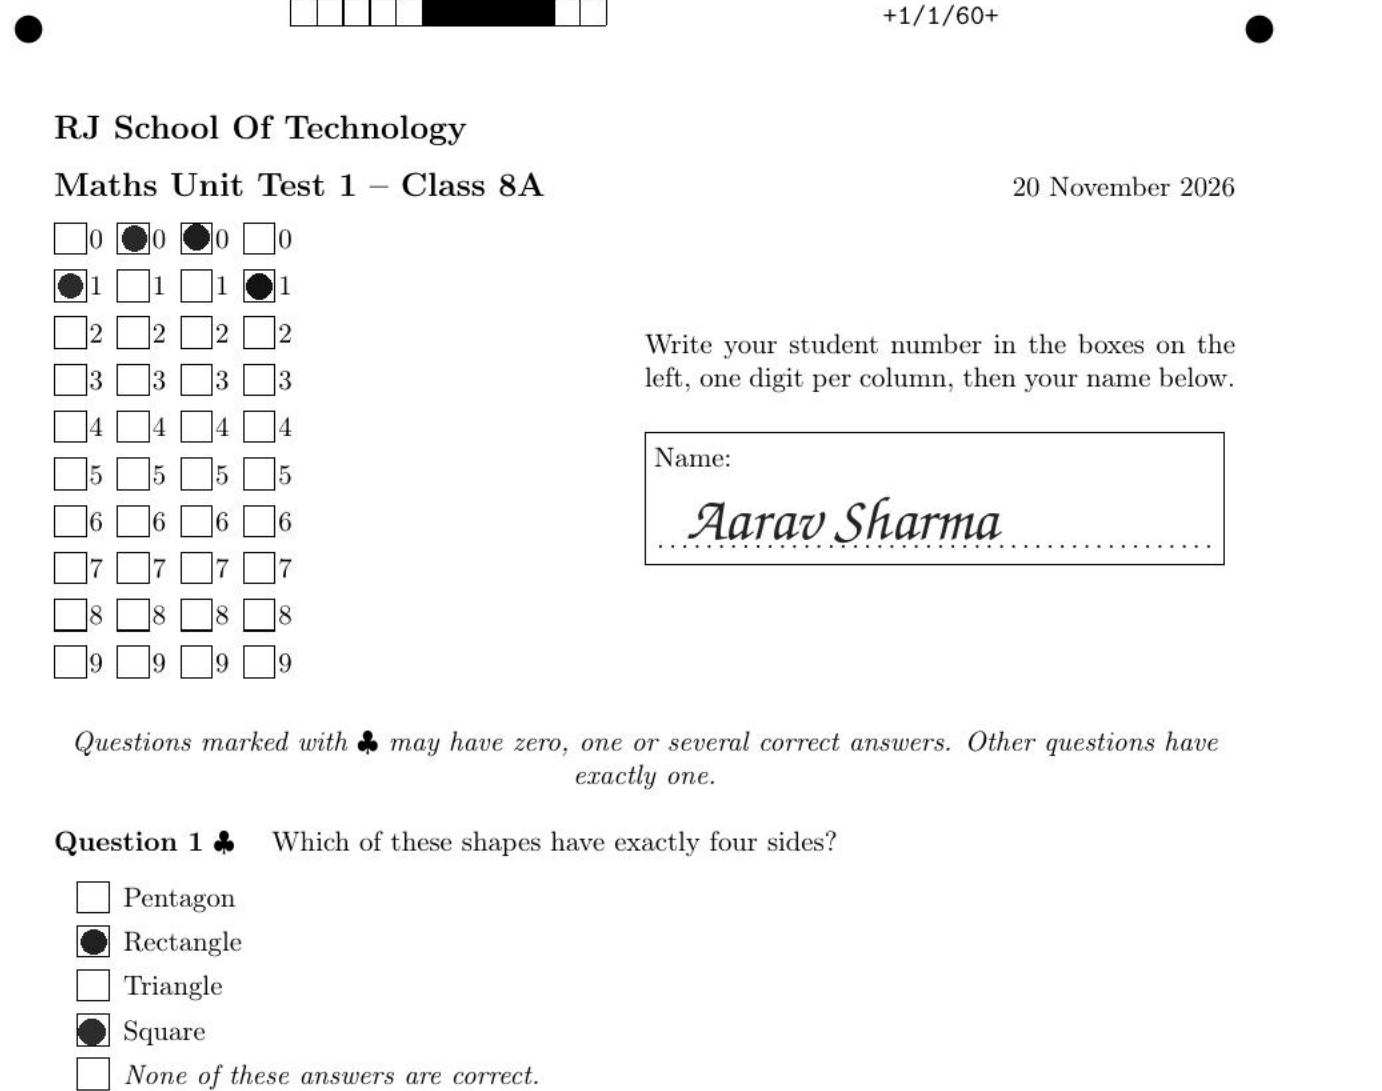
\includegraphics[width=0.78\linewidth]{screenshots/scan-sample}};
\end{center}

% ---------------------------------------------------------------------- step 5
\stephead{5}{after}{Upload scans}{Send the scanned pages to the portal; each one is read automatically.}\label{step:upload}

\begin{keep}
\begin{guidefig}{Upload scans, before the first upload.}
\begin{shot}[0.8\linewidth]{upload}
  \mk[nw]{drop}{1}\mk[nw]{photocopy}{2}
\end{shot}
\end{guidefig}
\begin{callouts}
  \item Drag your scan files onto this area, or click it to choose them. Several files at once are fine.
  \item \ui{Students wrote on photocopies}: tick this \emph{before} the first upload only if one printed paper was photocopied for the class.
\end{callouts}
\end{keep}

A progress box shows the pages being read, which takes a few seconds per page:

\begin{center}
\begin{shot}[0.55\linewidth]{upload-progress}\end{shot}
\end{center}

\begin{tip}[Messages from AMC]
The portal may show a message such as ``This page seems to be blank'', in AMC's words, with the file name. Press \ui{OK}: you will deal with such pages in the next step.
\end{tip}

When reading is done, five numbers sum up the result:

\begin{keep}
\begin{guidefig}{After the upload: the summary, and the next step waiting.}
\begin{shot}[0.85\linewidth]{upload-done}
  \mk[nw]{stats}{1}\mk[e]{badge}{2}\mk[w]{next}{3}
\end{shot}
\end{guidefig}
\begin{callouts}
  \item Pages read, complete copies, incomplete copies (a page missing), unreadable pages, and pages to check. Green is good; orange and red need you.
  \item The orange count on \ui{Check scans} is the number of things to look at.
  \item \ui{Next: Check scans}.
\end{callouts}
\end{keep}

% ---------------------------------------------------------------------- step 6
\stephead{6}{after}{Check scans}{Settle what the automatic reading couldn't, before marking.}\label{step:check}

Most pages need nothing. This step lists the few that do, in three kinds.

\begin{keep}
\begin{guidefig}{Check scans: an unreadable page, a missing page and two pages to check.}
\begin{shot}{check}
  \mk[nw]{failed}{1}\mk[n]{saw}{2}\mk[ne]{remove}{3}\mk[nw]{missing}{4}\mk[nw]{review}{5}\mk[nw]{preview}{6}
\end{shot}
\end{guidefig}
\begin{callouts}
  \item \textbf{Unreadable pages}: the portal couldn't recognise them as pages of this exam. Usually a blank back page, a page from another exam, or a page scanned crooked, too light or cut off.
  \item \ui{What AMC saw}: shows the page as the portal saw it, to understand why.
  \item The bin removes the page. If it belongs to the exam, scan it again (straight, 300\,dpi) and upload it.
  \item \textbf{Missing pages}: some pages of a copy came back, others didn't. Find the missing page in the pile, scan it and upload it in Upload scans. If it is really lost, the copy is marked with the pages it has.
  \item \textbf{Pages to check}: pages with a box whose darkness is close to the limit, for example a faint tick.
  \item The page being checked, with the boxes counted as ticked in green. Click a box there to change it.
\end{callouts}
\end{keep}

\subsubsection{Deciding the uncertain boxes}

\begin{keep}
\begin{guidefig}{Deciding an uncertain box: the zoomed box on the left, the whole page on the right.}
\begin{shot}{check-review}
  \mk[nw]{list}{1}\mk[nw]{row}{2}\mk[se]{done}{3}\mk[nw]{page}{4}
\end{shot}
\end{guidefig}
\begin{callouts}
  \item The pages to check, one after another.
  \item Each uncertain box, zoomed in, with how dark it is. Choose \ui{Ticked} or \ui{Not ticked} (or press \key{T} or \key{N}).
  \item \ui{Page done} (or \key{Enter}) moves to the next page.
  \item The whole page, to see the box in context.
\end{callouts}
\end{keep}

\begin{tip}[Many pages to check?]
\ui{Accept the rest as detected} settles all the remaining pages as the portal read them. If almost every page is ``to check'', the scans are probably very light or very dark: under \ui{Advanced: detection sensitivity} you can change how dark a box must be to count as ticked.
\end{tip}

When nothing is left, every number is green and the step gets a tick:

\begin{center}
\begin{shot}[0.8\linewidth]{check-clear}
  \hl{stats}
\end{shot}
\end{center}

% ---------------------------------------------------------------------- step 7
\stephead{7}{after}{Mark}{Turn the ticks into points and a mark for every copy.}\label{step:mark}

\begin{keep}
\begin{guidefig}{Mark: the checklist before marking.}
\begin{shot}[0.72\linewidth]{mark-before}
  \mk[nw]{list}{1}\mk[w]{go}{2}
\end{shot}
\end{guidefig}
\begin{callouts}
  \item Everything should be green: no unreadable, missing or uncertain pages.
  \item \ui{Compute marks}. It takes a few seconds.
\end{callouts}
\end{keep}

\begin{tip}
If problems remain, \ui{Mark anyway} still works, behind a warning that explains how each problem is treated.
\end{tip}

\begin{keep}
\begin{guidefig}{After marking: the summary, and the answers that broke a question's rules.}
\begin{shot}{mark-done}
  \mk[nw]{cards}{1}\mk[nw]{breaking}{2}\mk[w]{again}{3}
\end{shot}
\end{guidefig}
\begin{callouts}
  \item How many copies were marked, the mean, the median, the lowest and the highest mark.
  \item \textbf{Answers that break the rules}: for example two boxes ticked on a single-answer question. They score 0 by default. \ui{Open the page} lets you check the boxes were read correctly.
  \item \ui{Recompute marks}, after any change to the marking scheme, the answer key or a scan.
\end{callouts}
\end{keep}

Further down, \textbf{How each question did} shows, for each question, the share of students who got it right and how well it tells strong students from weak ones. A question that weaker students got right more often than stronger ones often has a \textbf{wrong answer key}: check it in Marking scheme.

\begin{center}
\begin{shot}[0.8\linewidth]{mark-stats}\end{shot}
\end{center}

% ---------------------------------------------------------------------- step 8
\stephead{8}{after}{Match students}{Put a student's name on each answer sheet.}\label{step:match}

\subsubsection{The class list}

Make the class list in any spreadsheet, with the column names on the first line and one student per line, and save it as \textbf{CSV (UTF-8)}. A student number column is what makes automatic matching possible:

\begin{center}
\begin{tabular}{@{}lll@{}}\toprule\texttt{id} & \texttt{surname} & \texttt{name}\\\midrule \texttt{1001} & Sharma & Aarav\\ \texttt{1002} & Patel & Diya\\ \ldots & & \\\bottomrule\end{tabular}
\end{center}

\begin{guidefig}{Match students, before loading the class list.}
\begin{shot}[0.72\linewidth]{match-start}
  \mk[nw]{drop}{1}
\end{shot}
\end{guidefig}

Drop the CSV file on the class-list area \badge{1}, or click it to choose the file. Then:

\begin{keep}
\begin{guidefig}{After loading the class list and matching automatically.}
\begin{shot}{match-auto}
  \mk[nw]{list}{1}\mk[nw]{key}{2}\mk[nw]{code}{3}\mk[w]{auto}{4}\mk[nw]{manual}{5}
\end{shot}
\end{guidefig}
\begin{callouts}
  \item The class list: 13 students here. \ui{Preview} shows it, \ui{Replace} loads a new version.
  \item \ui{Column with the student code}: the column holding the student numbers (\texttt{id} here).
  \item \ui{Code on the answer sheet}: the student number grid on the paper (\texttt{student}).
  \item \ui{Match automatically}. Here 11 of the 12 sheets were matched at once.
  \item The sheets left to \textbf{match by hand}.
\end{callouts}
\end{keep}

\subsubsection{Matching by hand}

A sheet stays unmatched when the number on it isn't in the class list, usually because the student ticked a wrong digit, or when there was no number grid. The portal shows the name the student wrote:

\begin{keep}
\begin{guidefig}{Matching by hand: copy 9 has the number 1019, which nobody has; the student wrote ``Arjun Das''.}
\begin{shot}[0.72\linewidth]{match-manual}
  \mk[nw]{name}{1}\mk[nw]{code}{2}\mk[w]{search}{3}\mk[w]{result}{4}\mk[e]{none}{5}
\end{shot}
\end{guidefig}
\begin{callouts}
  \item The name written on the sheet.
  \item The student number read on the sheet, and why it didn't match.
  \item Type part of the name or of the number\ldots
  \item \ldots{} and press \key{Enter} to match the highlighted student (\key{$\uparrow$}\,\key{$\downarrow$} choose another).
  \item \ui{Not in the class list}, for a student who isn't on your list.
\end{callouts}
\end{keep}

\begin{tip}
Students without a sheet yet are listed first: they are the likely ones. Matching a student who is already on another sheet moves them, and that other sheet goes back to the list to match.
\end{tip}

% ---------------------------------------------------------------------- step 9
\stephead{9}{after}{Export marks}{Get the marks out, as a spreadsheet.}\label{step:export}

\begin{keep}
\begin{guidefig}{Export marks: the summary, how the marks are spread, and the export settings.}
\begin{shot}{export}
  \mk[nw]{stats}{1}\mk[nw]{hist}{2}\mk[n]{format}{3}\mk[n]{ods}{4}\mk[w]{go}{5}
\end{shot}
\end{guidefig}
\begin{callouts}
  \item The same summary as in Mark.
  \item How many students got each mark.
  \item \ui{CSV}: a plain table, for any spreadsheet program or the school's system.
  \item \ui{ODS}: a LibreOffice spreadsheet with the points per question, and statistics if you want them.
  \item \ui{Export as CSV} (or ODS). Choose the order (by name, by mark\ldots) and whether to include absent students first.
\end{callouts}
\end{keep}

Lower on the page, the full table of marks can be sorted and searched before you export:

\begin{center}
\begin{shot}[0.7\linewidth]{export-table}
  \mk[w]{search}{1}
\end{shot}
\end{center}

\begin{guidefig}{After exporting: the CSV file opens in the preview panel; download it with the arrow.}
\begin{shot}{export-done}
  \mk[nw]{preview}{1}
\end{shot}
\end{guidefig}

Each line holds the copy number, the student's number and name, the final mark, and the points for each question.

\begin{careful}[Names missing?]
A sheet that isn't matched to a student is exported with its copy number only. Go back to Match students, then export again.
\end{careful}

% ---------------------------------------------------------------------- step 10
\stephead{10}{after}{Annotate}{Make each student's marked answer sheet, to give back.}\label{step:annotate}

\begin{keep}
\begin{guidefig}{Annotate: where the marks go, the files, the symbols on the boxes.}
\begin{shot}{annotate}
  \mk[nw]{where}{1}\mk[e]{position}{2}\mk[nw]{files}{3}\mk[nw]{symbols}{4}
\end{shot}
\end{guidefig}
\begin{callouts}
  \item \ui{On each sheet}: the header text at the top of each sheet (\texttt{\%s} is the mark, \texttt{\%m} what it is out of, \texttt{\%(name)} any class-list column).
  \item \ui{Marks for each question}: \ui{In one margin} keeps them clear of the symbol key (the default, \ui{In both margins}, can cover it).
  \item \ui{Files}: one PDF per student or one for the class, and how they are named.
  \item \ui{Symbols and key}: how each box is marked. \ui{Clear in black and white} gives each case its own shape, so the sheets stay readable when photocopied.
\end{callouts}
\end{keep}

Further down, choose a student under \ui{Preview one student} and press \ui{Preview}: their marked sheet opens in the preview panel.

\begin{guidefig}{A marked sheet: the name and mark at the top, each question's points in the margin, and a symbol on each box.}
\begin{shot}{annotate-preview}
  \mk[nw]{preview}{1}
\end{shot}
\end{guidefig}

When it looks right, press \ui{Annotate all sheets}, then \ui{Download all (zip)}.

\begin{guidefig}{All sheets made: download them in one zip file.}
\begin{shot}{annotate-done}
  \mk[w]{zip}{1}
\end{shot}
\end{guidefig}

\begin{tip}
File names show a copy number instead of a name when that sheet isn't matched to a student. After changing marks or matches, the step says \emph{Out of date}: annotate again.
\end{tip}

That's the whole journey: the exam now shows \emph{Exported} and a tick on every step.

% ====================================================================== 6
\section{Choosing a template}\label{sec:templates}

The template is chosen once, in the second page of \ui{New exam}. It decides how the paper looks and how you will edit it.

\subsection{The Starters}

\begin{panel}
\renewcommand{\arraystretch}{1.35}
\begin{tabularx}{\linewidth}{@{}>{\bfseries}p{36mm}X@{}}
Blank exam & A clean A4 paper with the school's name, a title line, the student number grid and a name box, then the questions. Questions are written in the \textbf{form}. \textbf{The best start for most exams}, and the one used in this guide.\\
RJ Style Paper Builder & A paper you \textbf{design from blocks}: logos, title lines, student details, instructions, the questions, and an \textbf{OMR answer sheet} of your own. For olympiad-style papers and printed answer sheets (\seesec{sec:builder}).\\
Blank exam, plain text & Questions typed in AMC's plain-text format, without the form: a line starting with \texttt{*} is a question, \texttt{+} a correct answer, \texttt{-} a wrong one. Quick for people who like typing, but the form, question banks and the Paper builder aren't available for it.\\
\end{tabularx}
\end{panel}

\subsection{AMC's examples}

The \ui{English}, \ui{French} and \ui{Other} groups hold the examples from AMC's documentation: different layouts, separate answer sheets, sheets printed with each student's name, scoring examples. They are good to see what AMC can do. Their questions live in one LaTeX file, so they suit teachers who know LaTeX. A preview shows one copy before you choose.

\begin{guidefig}{AMC's English examples, here ``Separate answers'' selected with its preview.}
\begin{shot}{gallery-amc}
  \mk[nw]{groups}{1}\mk[n]{card}{2}\mk[nw]{preview}{3}
\end{shot}
\end{guidefig}

\subsection{Answers on the paper, or a separate answer sheet?}

With the Blank exam you choose on the last page of the wizard (figure on page~\pageref{sec:create}):

\begin{panel}
\renewcommand{\arraystretch}{1.35}
\begin{tabularx}{\linewidth}{@{}>{\bfseries}p{40mm}X@{}}
On the question paper & Boxes next to each question. Natural for students, and nothing to copy across. Scan every page.\\
On a separate answer sheet & All boxes on one sheet at the end of each copy. Students work on the questions, then fill the sheet; you scan only the answer sheets. Better for long papers.\\
\end{tabularx}
\end{panel}

\begin{tip}
Tick \ui{Students write their student number in boxes} in both cases. It saves you typing names later: sheets are matched to the class list automatically.
\end{tip}

\subsection{The RJ Style Paper Builder}\label{sec:builder}

Choose \textbf{RJ Style Paper Builder} in the Starters. Its options page sets up the paper:

\begin{keep}
\begin{guidefig}{The RJ Style Paper Builder's options.}
\begin{shot}{wiz-builder}
  \mk[nw]{kind}{1}\mk[nw]{presets}{2}\mk[nw]{fields}{3}\mk[nw]{versions}{4}\mk[nw]{codes}{5}
\end{shot}
\end{guidefig}
\begin{callouts}
  \item The kind of paper: a separate OMR answer sheet, or answers on the question paper.
  \item A starting layout: \textbf{RJ Olympiad} (a full olympiad paper), \textbf{Simple} or \textbf{Blank}.
  \item The details printed on the paper: exam name, organiser, level, date, time, maximum marks.
  \item \ui{Versions of the paper}: how many different papers (A, B, C\ldots) to make. Each draws its own questions; you photocopy each version for part of the class.
  \item \ui{Paper codes}: letters, numbers or none.
\end{callouts}
\end{keep}

After creating it, open \ui{Questions} \textrightarrow{} \ui{Paper builder}. The page is made of \textbf{rows}; each row is split into \textbf{blocks} side by side, like a table.

\begin{keep}
\begin{guidefig}{The Paper builder: the title block selected, its settings on the right.}
\begin{shot}{builder}
  \mk[nw]{tabs}{1}\mk[nw]{row}{2}\mk[s]{block}{3}\mk[nw]{side}{4}
\end{shot}
\end{guidefig}
\begin{callouts}
  \item The parts: \ui{Question paper}, \ui{Answer sheet}, \ui{Instructions}, \ui{Details}, \ui{Sections}, \ui{Versions and page}.
  \item A row, with buttons to move it, delete it or add a column.
  \item A block. Click it to change it; drag it to move it.
  \item The selected block's settings: its kind, width, border, alignment and content.
\end{callouts}
\end{keep}

The \ui{Answer sheet} tab designs the OMR sheet the same way: student details, the student number grid, signature boxes, and the answer boxes for every question.

\begin{guidefig}{The Answer sheet tab.}
\begin{shot}[0.9\linewidth]{builder-omr}
\end{shot}
\end{guidefig}

\begin{tip}
Every change is saved and kept in History. Press \ui{Build preview} to see the result. A design that can't be printed (no questions block, or an answer sheet without answer boxes) is flagged, and the build waits until it is fixed.
\end{tip}

\subsection{Sections: which questions go on each paper}\label{sec:sections}

In any exam, \ui{Questions} \textrightarrow{} \ui{Paper builder} (or \ui{Sections} in the RJ builder) groups the questions into \textbf{sections}, each printed under its own heading. For each section you can set:

\begin{itemize}
  \item \textbf{Questions per copy}: all of them, or fewer, drawn at random for each copy (``10 of 15 per copy'');
  \item \textbf{shuffle} the questions in each copy, \textbf{columns} (1 to 4), \textbf{start on a new page};
  \item a \textbf{heading} and \textbf{instructions} printed above the questions.
\end{itemize}

\begin{keep}
\begin{guidefig}{Sections in Maths Unit Test 2: one section came from a bank group, another from ticked bank questions.}
\begin{shot}{paper-design}
  \mk[w]{add}{1}\mk[nw]{breaks}{2}\mk[e]{edit}{3}
\end{shot}
\end{guidefig}
\begin{callouts}
  \item \ui{Add a section}.
  \item \ui{Page breaks}: whether each section starts on a new page.
  \item \ui{Edit} a section: its heading, how many questions per copy, shuffling, columns.
\end{callouts}
\end{keep}

\subsection{Your own templates}\label{sec:mytemplates}

When an exam's paper is just right, make it a template: \ui{Exam settings} \textrightarrow{} \ui{Save as a template\ldots}. It keeps the questions, sections, paper and settings, without scans or marks. Next time, choose it in \ui{New exam} under \ui{My templates} (figure on page~\pageref{sec:settings}).

\subsection{Which one should I choose?}

\begin{panel}
\renewcommand{\arraystretch}{1.35}
\begin{tabularx}{\linewidth}{@{}X>{\bfseries}p{62mm}@{}}
\toprule
\normalfont\bfseries If you want\ldots & Choose\\
\midrule
A normal class test, quickly & Blank exam, answers on the paper\\
A long paper, students answer on one sheet & Blank exam, separate answer sheet\\
An olympiad-style paper, logos, an OMR sheet of your design & RJ Style Paper Builder\\
Several versions (A, B, C) photocopied & RJ Style Paper Builder, versions\\
The same layout as last term & My templates\\
To write everything in LaTeX yourself & An AMC example, or Blank exam with the LaTeX tab\\
\bottomrule
\end{tabularx}
\end{panel}

% ====================================================================== 7
\section{Managing question banks}\label{sec:banks}

A \textbf{question bank} is your own collection of questions to use again in any exam: last year's best questions, a chapter's worth of practice questions, questions shared by a colleague. Only you see your banks.

\begin{itemize}
  \item A bank keeps its questions in \textbf{groups}, such as \emph{Arithmetic}, \emph{Geometry}, \emph{Algebra}, the way an exam keeps them in sections.
  \item Each question can have a \textbf{difficulty} (easy, medium, hard) and \textbf{tags}, to find it again.
  \item An exam gets a \textbf{copy} of a bank question, not a link. Changing the copy doesn't change the bank, and the other way round, until \emph{you} choose to bring the change across (\seesec{sec:bank-copies}).
\end{itemize}

\subsection{Create a bank}

Open \ui{Question banks} at the top of any page.

\begin{keep}
\begin{guidefig}{The Question banks page, before the first bank.}
\begin{shot}[0.9\linewidth]{banks-empty}
  \mk[s]{new}{1}\mk[s]{import}{2}
\end{shot}
\end{guidefig}
\begin{callouts}
  \item \ui{New bank}.
  \item \ui{Import a bank\ldots}: a bank someone downloaded as a zip file (\seesec{sec:bank-move}).
\end{callouts}
\end{keep}

\begin{guidefig}{A name and a short description for the bank.}
\begin{shot}[0.52\linewidth]{bank-new}
  \mk[w]{name}{1}\mk[e]{ok}{2}
\end{shot}
\end{guidefig}

\subsection{Put questions in}

There are three ways, and you can mix them.

\subsubsection{Type them in the bank}

A bank's page looks like an exam's Questions step: groups and questions on the left, the same form on the right.

\begin{keep}
\begin{guidefig}{A bank with three groups; the question ``perimeter'' open in the form.}
\begin{shot}{bank-page}
  \mk[ne]{list}{1}\mk[n]{groups}{2}\mk[nw]{meta}{3}\mk[nw]{search}{4}\mk[n]{history}{5}
\end{shot}
\end{guidefig}
\begin{callouts}
  \item The groups and their questions. \ui{+ Group} adds a group; the \texttt{+} on a group adds a question to it; the pencil renames it or sets its instructions and default scoring.
  \item A group, here \emph{Geometry}, with its 4 questions.
  \item The question's \ui{Difficulty}, its \ui{Tags} (separated by commas), and \ui{Archived} to stop offering it.
  \item Search and filters: words, difficulty, kind, tag, and when the question was last printed.
  \item \ui{History}, \ui{Import LaTeX\ldots}, and the \ui{$\cdots$} menu (rename, describe, download as a zip, delete).
\end{callouts}
\end{keep}

\subsubsection{Import a LaTeX file}

If you have questions in LaTeX files where each question is an \verb|\element{group}{...}| block (as in RJ question files), \ui{Import LaTeX\ldots} reads them all at once, with their figures. Each \verb|\element| group becomes a group of the bank.

\begin{guidefig}{Importing a LaTeX file of questions.}
\begin{shot}[0.55\linewidth]{bank-import}
  \mk[w]{file}{1}\mk[e]{go}{2}
\end{shot}
\end{guidefig}

\subsubsection{Save questions from an exam}

In an exam, \ui{Save to a bank\ldots} (above a question in the form) copies that question into a bank group; in the Paper builder, a section can be saved as a whole group; and \ui{Exam settings} \textrightarrow{} \ui{Save as a bank\ldots} makes a new bank from a whole exam, with one group per section.

\begin{guidefig}{Saving one question of an exam into a bank.}
\begin{shot}[0.52\linewidth]{save-to-bank}\end{shot}
\end{guidefig}

\subsection{Use bank questions in an exam}\label{sec:bank-use}

In the exam's Questions step, press \ui{From a bank\ldots} above the list of questions.

\begin{keep}
\begin{guidefig}{Adding questions from a bank.}
\begin{shot}{picker}
  \mk[nw]{bank}{1}\mk[nw]{group}{2}\mk[w]{modes}{3}\mk[nw]{list}{4}\mk[n]{add}{5}
\end{shot}
\end{guidefig}
\begin{callouts}
  \item The bank\ldots
  \item \ldots{} and the group to take questions from.
  \item What to add:
    \begin{itemize}
      \item \textbf{the whole group, as a new section}: its title becomes the section's heading;
      \item \textbf{the whole group, into a section} you choose;
      \item \textbf{the questions ticked below};
      \item \textbf{by a blueprint}, such as ``3 easy + 5 medium from Algebra'';
      \item \textbf{a number picked at random} from the questions shown.
    \end{itemize}
  \item The group's questions, with their difficulty, tags and when they were last printed.
  \item \ui{Add to the exam}.
\end{callouts}
\end{keep}

\begin{guidefig}{Two ticked questions from the Geometry group, going into the section ``general''.}
\begin{shot}{picker-ticked}
  \mk[w]{mode}{1}\mk[w]{ticks}{2}\mk[n]{add}{3}
\end{shot}
\end{guidefig}

\begin{keep}
\begin{guidefig}{A blueprint: 2 medium questions from Algebra, picked at random and shown before they are added.}
\begin{shot}{picker-blueprint}
  \mk[nw]{rows}{1}\mk[n]{pick}{2}\mk[nw]{chosen}{3}
\end{shot}
\end{guidefig}
\begin{callouts}
  \item Rows of ``how many, which difficulty, from which group, with which tag''. Add rows for a mix.
  \item \ui{Pick} draws the questions (\ui{Pick again} for others).
  \item The questions drawn, to review before \ui{Add to the exam}.
\end{callouts}
\end{keep}

\begin{tip}
Macros and packages that the questions need come with them. A question the exam already has isn't added twice, and a question whose name is already used gets a new name in the copy.
\end{tip}

\subsection{When a question changes: copies and updates}\label{sec:bank-copies}

Suppose you improve a question in the bank after copying it into an exam. The exam's copy notices, and tells you:

\begin{keep}
\begin{guidefig}{The bank's question changed: the exam's copy says \emph{Bank updated}.}
\begin{shot}[0.72\linewidth]{copies-status}
  \mk[nw]{strip}{1}\mk[e]{badge}{2}\mk[w]{origin}{3}\mk[e]{compare}{4}
\end{shot}
\end{guidefig}
\begin{callouts}
  \item A note above the questions when copies differ from their bank questions; \ui{Review\ldots} lists them.
  \item The question's status in the list.
  \item Where the copy came from.
  \item \ui{Compare\ldots} shows the difference and the choices.
\end{callouts}
\end{keep}

\begin{keep}
\begin{guidefig}{Comparing: the bank added ``in centimetres''.}
\begin{shot}{compare}
  \mk[nw]{diff}{1}\mk[n]{keep}{2}\mk[n]{take}{3}
\end{shot}
\end{guidefig}
\begin{callouts}
  \item What changed, line by line.
  \item \ui{Keep this exam's}: leave the copy as it is; this bank version won't be offered again.
  \item \ui{Take the bank's version}: the copy becomes the bank's question.
\end{callouts}
\end{keep}

If you changed the copy in the exam instead, the choice is \ui{Update the bank's copy}; if both changed, \ui{Combine both}. Nothing changes until you choose. Once an exam is printed, only answer-key and scoring fixes can be taken from a bank.

\begin{panel}
\renewcommand{\arraystretch}{1.3}\small
\begin{tabularx}{\linewidth}{@{}>{\bfseries}p{52mm}X@{}}
Up to date & The copy and the bank question are the same.\\
Bank updated & The bank's question changed since the copy was made.\\
Edited here & The exam's copy was changed.\\
Both changed & Both were changed.\\
Bank's newer version set aside & You chose \emph{Keep this exam's}.\\
Not in the bank any more & The bank question was deleted.\\
\end{tabularx}
\end{panel}

\subsection{Find questions}

The search box on the \ui{Question banks} page searches \textbf{all your banks} at once: words of the question, its name or its tags. The start of a word is enough: \emph{quadr} finds \emph{quadratic}. Click a result to open it in its bank.

\begin{guidefig}{Searching all banks for ``square''.}
\begin{shot}[0.9\linewidth]{bank-search}
  \mk[nw]{search}{1}\mk[nw]{results}{2}
\end{shot}
\end{guidefig}

\begin{itemize}
  \item A bank question shows the exams that \textbf{printed} it, and how many times. Filters such as \emph{never printed} or \emph{not printed for a year} help avoid repeating last year's paper.
  \item After an exam is marked, a bank question also shows \textbf{how it did}: the share of students who got it right, over every exam that used it.
  \item \textbf{Archive} a question you no longer want to offer: it stays in the bank and in old exams, but is hidden from \ui{From a bank\ldots}.
\end{itemize}

\subsection{Move or share a bank}\label{sec:bank-move}

In a bank's \ui{$\cdots$} menu, \ui{Download as a zip (with its history)} saves the whole bank. On the Question banks page, \ui{Import a bank\ldots} reads such a zip as a new bank of your own: to move a bank to another computer, or to give a colleague a copy.

% ====================================================================== 8
\section{The safety net and housekeeping}\label{sec:safety}

\subsection{History: every save is kept}\label{sec:history}

Every change to an exam is kept as a version, for good: who saved it, when, and what changed. Open \ui{History} at the top of the Questions step (also in the Paper builder and on a bank's page).

\begin{keep}
\begin{guidefig}{History of the whole exam; a version selected, with what it changed.}
\begin{shot}{history}
  \mk[nw]{file}{1}\mk[nw]{list}{2}
\end{shot}
\end{guidefig}
\begin{callouts}
  \item Show the history of the whole exam, or of one file.
  \item A version. Its changes are shown in words and line by line, with three ways back: \ui{Restore the exam to this version}, \ui{Restore only this file}, or \ui{Undo this change}. Every restore can itself be undone.
\end{callouts}
\end{keep}

\begin{tip}
\ui{Build this version} shows how the paper looked in an older version, without changing anything. \ui{Name this version} gives it a name, such as ``Checked by the head of department''. Printing names the version that was printed.
\end{tip}

\subsection{Trash: deleted exams come back}

A deleted exam (or bank) stays in the \ui{Trash} for \textbf{30 days}, with its history. Open \ui{Trash} on the Exams page and press \ui{Restore}.

\begin{guidefig}{The Trash.}
\begin{shot}[0.55\linewidth]{trash}
  \mk[e]{restore}{1}
\end{shot}
\end{guidefig}

\subsection{Exam settings}\label{sec:settings}

\ui{Exam settings}, at the bottom of the step list, gathers what concerns the exam as a whole.

\begin{keep}
\begin{guidefig}{Exam settings.}
\begin{shot}{exam-settings}
  \mk[n]{rename}{1}\mk[w]{duplicate}{2}\mk[w]{bank}{3}\mk[w]{template}{4}\mk[w]{download}{5}
\end{shot}
\end{guidefig}
\begin{callouts}
  \item \ui{Rename} the exam. Below it: the class, subject and date, and the LaTeX engine (leave \emph{pdflatex}).
  \item \ui{Duplicate}: a full copy of the exam. The safe way to make a new exam from a printed one.
  \item \ui{Save as a bank\ldots}: a new question bank with a group per section (\seesec{sec:banks}).
  \item \ui{Save as a template\ldots} (\seesec{sec:mytemplates}).
  \item \ui{Download}: everything in the exam as a zip file, for your own backup.
\end{callouts}
\end{keep}
Further down the page: the exam's activity, \ui{Unlock\ldots}{} and \ui{Delete}.

\subsection{Your Exams page, later on}

As you add exams, each one gets a card that says where it stands and what comes next.

\begin{keep}
\begin{guidefig}{The Exams page with three exams.}
\begin{shot}{dash}
  \mk[n]{search}{1}\mk[n]{filters}{2}\mk[w]{card}{3}\mk[n]{menu}{4}
\end{shot}
\end{guidefig}
\begin{callouts}
  \item Search by name, class or subject.
  \item Filter by class or state, and sort.
  \item An exam's card: its class, subject and date, its state (\emph{Draft}, \emph{Printed}, \emph{Exported}\ldots), a bar showing its progress through the ten steps, and the next thing to do. \ui{Continue} opens it there.
  \item More: class, subject and date; \ui{Rename}; \ui{Duplicate}; \ui{Download as zip}; \ui{Archive} (hide old exams without deleting them); \ui{Delete}.
\end{callouts}
\end{keep}

\subsection{The built-in guide}

\ui{Guide} at the top opens the portal's own help: \ui{About this step}, \ui{The full guide} and \ui{Take the tour}. Each step's page ends with its common problems and their fixes.

\begin{guidefig}{The Guide menu, and the help page of a step.}
\begin{minipage}[t]{0.3\linewidth}\vspace{0pt}
\begin{shot}{guide-menu}\end{shot}
\end{minipage}\hfill
\begin{minipage}[t]{0.66\linewidth}\vspace{0pt}
\begin{shot}{guide-page}\end{shot}
\end{minipage}
\end{guidefig}

% ====================================================================== 9
\section{Problems and fixes}\label{sec:problems}

\begin{panel}
\small\renewcommand{\arraystretch}{1.3}
\begin{tabularx}{\linewidth}{@{}>{\bfseries\raggedright}p{50mm}X@{}}
\toprule
Problem & What to do\\
\midrule
The preview or papers don't build & Read the red message: it names the question and the line. Look for a missing \texttt{\}} or a \texttt{\%} \texttt{\&} \texttt{\#} \texttt{\_} without a backslash. History can bring back the last version that built (marked \emph{built OK}).\\
A picture doesn't appear & Add it with \ui{Insert an image} in the form, or \ui{Add a file} in the LaTeX tab, and use exactly the same file name.\\
A box isn't outlined in the layout check & It was drawn without AMC's commands (for example as a picture). Use the form's answers.\\
Many pages are unreadable & Print at 100\,\%, scan at 300\,dpi, straight, with all four corner dots on the page.\\
Almost every page is ``to check'' & The scans are very light or dark. Check scans \textrightarrow{} \ui{Advanced: detection sensitivity}.\\
A student filled a box completely & A fully black box counts as \emph{cancelled}, not ticked. Decide it by hand in Check scans if needed.\\
A sheet doesn't match automatically & The student ticked a wrong digit, or their number isn't in the class list. Match it by hand by typing the name (page~\pageref{step:match}).\\
Leading zeros in student numbers & They don't matter: 0123 matches 123.\\
``The class list can't be read'' & Save it as \textbf{CSV (UTF-8)} from your spreadsheet, with column names on the first line.\\
Marks, export or sheets say \emph{Out of date} & Something changed after marking. Recompute marks, then export and annotate again.\\
A wrong answer key, found after the exam & Marking scheme: click the right answer to make it correct (allowed after printing), then recompute marks.\\
A question was wrong or unclear & Marking scheme \textrightarrow{} \ui{Scoring\ldots} \textrightarrow{} \ui{Full marks for everyone} or \ui{Not counted}.\\
A question must change after printing & Better: \ui{Duplicate} the exam and change the copy. \ui{Unlock\ldots} removes scans and marks, and printed papers no longer match.\\
I deleted an exam by mistake & Exams page \textrightarrow{} \ui{Trash} \textrightarrow{} \ui{Restore} (within 30 days).\\
I broke something while editing & History: restore the file or the whole exam, or undo one change.\\
I forgot my password & Ask the portal's administrator to reset it.\\
``This file was changed since you opened it'' & The same exam was saved from another tab. Keep your version (the other stays in History), or load theirs.\\
\bottomrule
\end{tabularx}
\end{panel}

% ====================================================================== 10
\section{Checklist}\label{sec:checklist}

Print this page and keep it next to you for your first exams.

\newcommand\cb{\tikz[baseline=-0.6ex]\node[draw=muted,line width=0.6pt,minimum size=3mm,inner sep=0pt,rounded corners=0.6pt]{};}
\setlist[itemize,2]{label=\cb,leftmargin=6mm}
\begin{panel}[colframe=before,boxrule=1pt,title={\bfseries Before the exam},colbacktitle=before,coltitle=white]
\begin{itemize}[label=\cb]
  \item New exam: name, class, subject, date; template (Blank exam if unsure); student number boxes ticked; copies = class + spares.
  \item Questions: every question written, the correct answers ticked (green); title and date set in the LaTeX tab.
  \item \ui{Build preview}: read the paper once from top to bottom.
  \item Marking scheme: default scoring saved; \ui{Out of} set.
  \item Papers: built; layout checked; \ui{Looks correct}.
  \item Print: PDFs saved; printed on A4 at \textbf{100\,\%}, every copy, corner dots on the paper.
\end{itemize}
\end{panel}

\begin{panel}[colframe=warn,boxrule=1pt,title={\bfseries Exam day},colbacktitle=warn,coltitle=white]
\begin{itemize}[label=\cb]
  \item Students use a dark pen, write their student number in the grid and their name in the box.
  \item To cancel a tick, fill the box completely.
  \item Collect every page of every copy.
\end{itemize}
\end{panel}

\begin{panel}[colframe=after,boxrule=1pt,title={\bfseries After the exam},colbacktitle=after,coltitle=white]
\begin{itemize}[label=\cb]
  \item Scan at 300\,dpi, greyscale or black and white, straight.
  \item Upload scans; press \ui{OK} on any AMC message.
  \item Check scans: unreadable pages removed or rescanned; missing pages uploaded; uncertain boxes decided.
  \item Mark: \ui{Compute marks}; look at \emph{answers that break the rules} and \emph{how each question did}.
  \item Match students: class list (CSV) loaded; \ui{Match automatically}; the rest by hand.
  \item Export marks: CSV or ODS downloaded.
  \item Annotate: one student previewed; all sheets annotated; zip downloaded.
  \item Any later change \textrightarrow{} recompute marks, export and annotate again.
\end{itemize}
\end{panel}

\vfill
\begin{center}\small\color{muted}
AMC web portal \textbullet{} \portal{} \textbullet{} built on Auto Multiple Choice (\href{https://www.auto-multiple-choice.net}{auto-multiple-choice.net}), free software under the GNU GPL.
\end{center}

\end{document}
